\documentclass[a4paper]{article}
\usepackage[english]{babel}
\usepackage[a4paper,top=2cm,bottom=2cm,left=2cm,right=2cm,marginparwidth=1.75cm]{geometry}
\usepackage{amsmath}
\usepackage{amsfonts}
\usepackage{amssymb}
\usepackage{graphicx}
\usepackage[colorlinks=true, allcolors=blue]{hyperref}
\usepackage{xcolor}
\usepackage{enumerate}
\usepackage{minted}
\usepackage{listings}
\renewcommand{\thesubsection}{\thesection.\alph{subsection}}
\lstset{
    basicstyle=\small\color{purple}\ttfamily,
    columns=flexible,
    breaklines=true,
}
\setlength\parindent{0pt}

\title{\textbf{Computer Networks} \\
      Assignment-1 \\
}

\author{\textsc{Himanshu Gaurav Singh } \\
    2019CS10358
}

\newcommand{\nl}{\vspace{0.2cm}\\}
\newcommand{\nln}{\vspace{0.2cm}}

\begin{document}

\maketitle
\tableofcontents

\section{Networking Tools}

\subsection{IP-address of personal machine}
Ran the command \textit{ipconfig getifaddr en0} to get the IP address of the machine - \textbf{10.184.20.241}. This was when I was logged in to IITD-Wifi. For my personal mobile phone hotspot (ISP-Reliance Jio), the IP address turns out to be \textbf{192.168.43.172}.\\
The IP address changed on changing the ISP. This is reasonable since it is the router that assigns an IP address to the interface between them.

\subsection{IP-address of various websites}
Ran the command \texttt{nslookup \textless domain-name\textgreater} to get the IP address associated with the websites. \\
On using the default DNS server for the ISP, the IP addresses come as follows - \\
\begin{center}
    \begin{tabular}{|c|c|c|}
        \hline
        Webpage & RELIANCE-JIO  & IITD-WIFI  \\  
        \hline
        www.google.com     & 142.250.77.206   & 142.250.182.174   \\ 
        \hline
        www.facebook.com       &  157.240.198.35  & 31.13.79.35  \\  
        \hline
    \end{tabular}
\end{center}

On using the Google public DNS, the results are - \\
\begin{center}
    \begin{tabular}{|c|c|c|}
        \hline
        Webpage & RELIANCE-JIO  & IITD-WIFI  \\  
        \hline
        www.google.com  & 142.250.195.14   &  142.250.193.238   \\ 
        \hline
        www.facebook.com       &  157.240.198.35 & 157.240.16.35  \\  
        \hline
    \end{tabular}
\end{center}
\subsubsection{Explanation}
\begin{itemize}
    \item Mostly(but not always), the change is in the last two sections of the IP address.
    \item This is happening probably because different DNS servers point to different host servers attached to the same domain name. It is likely that popular websites such as those of Google and Facebook have multiple servers.
\end{itemize}
\subsection{Ping}
Ran the command \texttt{ping -s \textless size\textgreater  -m \textless ttl-value\textgreater  \textless domain-name\textgreater}. \\
I did a binary-search for the maximum length of the packets and the minimum ttl value by repeatedly running the above command. 
The results for the minimum TTL value for which the packet could be sent and the maximum size of the packet that could be sent are as follows :
\begin{center}
    \begin{tabular}{|c|c|c|}
        \hline
        Domain-name & Minimum TTL  & Maximum packet size(bytes)  \\
        \hline
        www.iitd.ac.in & 4  & 8184 \\
        \hline
        www.google.com &  10   & 68  \\ 
        \hline
        www.facebook.com    &  12  & 1472  \\  
        \hline
    \end{tabular}
\end{center}
The packet size here excludes the header of size 8 bytes of the ICMP packet.
\begin{enumerate}
    \item The lower value of TTL for iitd.ac.in is evident since I was logged on to IITD-WiFi itself implying vicinity within the network to the IITD server. 
    \item Regarding the maximum packet size, for the IITD server, the maximum packet size  that could be sent by my machine, was $8192(2^{13})$. 
    \item The limit of 1472 bytes for facebook.com is probably due to the a cap of 1500 bytes on MTU( Maximum Transmission Unit) over the Ethernet. It corresponds to 1500 - 8 (ICMP header) - 20( IP header) = 1472 bytes.
    \item Thus, it is evident that maximum packet size might depend upon the number of routers in between the client and server apart from system specification. Probably, different routers/end-systems have different limitations over the size of the packets they send. Over and above all, we can send messages of at most total length 65536 bytes using IPv4.
\end{enumerate}

\subsection{Traceroute}
Ran the command \texttt{traceroute iitd.ac.in}
\subsubsection{www.iitd.ac.in}
Using personal hotspot (Reliance-JIO), the traceroute comes out as follows:
\begin{lstlisting}
traceroute to iitd.ac.in (103.27.9.24), 64 hops max, 52 byte packets
 1  192.168.43.1 (192.168.43.1)  1032.835 ms  5.549 ms  7.418 ms
 2  * * *
 3  10.71.83.34 (10.71.83.34)  206.575 ms  41.420 ms
    10.71.83.50 (10.71.83.50)  59.662 ms
 4  172.26.100.119 (172.26.100.119)  28.985 ms  73.069 ms  35.736 ms
 5  172.26.100.102 (172.26.100.102)  64.987 ms
    172.26.100.103 (172.26.100.103)  57.922 ms  46.272 ms
 6  192.168.44.26 (192.168.44.26)  38.798 ms
    192.168.44.28 (192.168.44.28)  59.328 ms
    192.168.44.22 (192.168.44.22)  42.704 ms
 7  192.168.44.25 (192.168.44.25)  57.403 ms
    192.168.44.29 (192.168.44.29)  63.647 ms
    192.168.44.23 (192.168.44.23)  37.225 ms
 8  172.26.14.73 (172.26.14.73)  63.038 ms
    172.16.26.5 (172.16.26.5)  64.028 ms
    172.26.14.73 (172.26.14.73)  47.789 ms
 9  172.16.18.0 (172.16.18.0)  47.890 ms  38.507 ms  42.070 ms
10  115.254.77.34 (115.254.77.34)  64.113 ms  71.759 ms
    115.110.210.37.static-delhi.vsnl.net.in (115.110.210.37)  27.637 ms
11  * * 115.255.253.18 (115.255.253.18)  87.734 ms
12  14.140.210.22.static-delhi-vsnl.net.in (14.140.210.22)  65.979 ms
    115.249.198.97 (115.249.198.97)  102.746 ms  111.101 ms
13  * * *
14  * * *
15  * * *
..........
64  * * * 
\end{lstlisting}
Following is the result of tracing a path to iitd.ac.in while being logged on to IIT-D Wifi.
\begin{lstlisting}
traceroute to iitd.ac.in (10.10.211.212), 64 hops max, 52 byte packets
 1  10.194.0.14 (10.194.0.14)  2.368 ms  1.804 ms  1.705 ms
 2  10.254.238.5 (10.254.238.5)  2.560 ms  2.251 ms  2.126 ms
 3  10.254.236.22 (10.254.236.22)  1.995 ms  2.208 ms
    10.254.236.14 (10.254.236.14)  2.640 ms
 4  www.iitd.ac.in (10.10.211.212)  1.768 ms  1.768 ms  2.036 ms
\end{lstlisting}
The short path is reasonable since the corresponding routers are reasonably close in the network. \\
\subsubsection{\texttt{www.google.com}}
Following is the route when the client machine used IITD-WiFi. \\
\begin{lstlisting}
traceroute to google.com (142.250.192.174), 64 hops max, 52 byte packets
 1  10.194.0.14 (10.194.0.14)  2.936 ms  1.364 ms  1.565 ms
 2  10.254.238.1 (10.254.238.1)  1.738 ms  1.748 ms  1.627 ms
 3  10.255.1.34 (10.255.1.34)  2.046 ms  1.911 ms  1.748 ms
 4  10.119.233.65 (10.119.233.65)  2.207 ms  2.168 ms  1.858 ms
 5  10.1.207.69 (10.1.207.69)  3.532 ms  3.720 ms  3.613 ms
 6  10.119.234.162 (10.119.234.162)  3.759 ms  4.236 ms  4.880 ms
 7  72.14.194.160 (72.14.194.160)  4.042 ms
    72.14.195.56 (72.14.195.56)  4.632 ms  4.408 ms
 8  74.125.243.97 (74.125.243.97)  5.698 ms  6.752 ms  5.975 ms
 9  172.253.73.195 (172.253.73.195)  5.387 ms  5.374 ms  5.305 ms
10  del11s11-in-f14.1e100.net (142.250.192.174)  5.221 ms  5.462 ms  5.034 ms
\end{lstlisting}

Following is the route when personal smartphone hotspot is used. \\
\begin{lstlisting}
traceroute to google.com (142.250.77.238), 64 hops max, 52 byte packets
 1  192.168.43.1 (192.168.43.1)  3.055 ms  2.826 ms  2.568 ms
 2  * * *
 3  10.71.83.34 (10.71.83.34)  158.438 ms  60.948 ms  59.493 ms
 4  172.26.100.119 (172.26.100.119)  60.005 ms  60.113 ms  58.518 ms
 5  172.26.100.103 (172.26.100.103)  60.136 ms  46.796 ms
    172.26.100.102 (172.26.100.102)  59.396 ms
 6  192.168.44.22 (192.168.44.22)  46.309 ms
    192.168.44.26 (192.168.44.26)  28.829 ms
    192.168.44.22 (192.168.44.22)  30.452 ms
 7  192.168.44.29 (192.168.44.29)  99.432 ms  42.589 ms
    192.168.44.27 (192.168.44.27)  283.440 ms
 8  172.16.26.5 (172.16.26.5)  65.128 ms
    172.16.18.33 (172.16.18.33)  62.436 ms  57.711 ms
 9  172.16.26.2 (172.16.26.2)  56.066 ms
    172.16.18.2 (172.16.18.2)  57.201 ms
    172.16.26.0 (172.16.26.0)  66.966 ms
10  142.250.168.56 (142.250.168.56)  66.164 ms  55.939 ms
    142.250.47.144 (142.250.47.144)  35.637 ms
11  * * *
12  72.14.233.30 (72.14.233.30)  73.834 ms
    64.233.174.70 (64.233.174.70)  316.269 ms
    142.251.52.210 (142.251.52.210)  30.268 ms
13  142.251.54.77 (142.251.54.77)  37.824 ms
    108.170.251.123 (108.170.251.123)  39.945 ms
    del11s09-in-f14.1e100.net (142.250.77.238)  61.703 ms
\end{lstlisting}
\subsubsection{Observations}
\begin{enumerate}
    \item Running \texttt{traceroute} multiple times gives different routes each time, which is reasonable since there can be several routes to the same end-system in the network.
    \item For the traceroute to IIT-D server, several of the first IP addresses are private addresses of the smartphone/local networks. After that, there are addresses belonging to Reliance(the ISP)(115.254.77.34). After that, we do not get any response, probably because packets to IIT-D servers are being blocked.
    \item In this case, 192.168.43.1 is the IP address of my smartphone. Observe that some of the routers in the path(hop 5 and 11) did not respond back, probably due to the smaller TTL value of the packet they sent. \texttt{traceroute} uses UDP-datagrams by default which are unreliable in general.
    \item In the case of IITD-WiFi, there were several private IP addresses, probably IIT-D servers followed by IP addresses belonging to Google. This shows that some  Google-owned routers probably share a direct connection to one of the IIT-D router.
\end{enumerate}
\subsubsection{Observations regarding IPv6}
\begin{enumerate}
    \item \texttt{traceroute} uses IPv4 by default. To use IPv6, run the command \texttt{traceroute6}.
    \item \texttt{iitd.ac.in} does not respond to IPv6 protocol. The message \texttt{traceroute6:nodename nor servname provided, or not known} is received. Running \texttt{traceroute6 google.com} while being logged on to IITD-WiFi gives \texttt{connect:No route to host}.
    Evidently, IITD routers and end-systems do not support IPv6.
    \item Running the above command while using personal hotspot gave the following result
    \begin{lstlisting}
traceroute6 to google.com (2404:6800:4002:81f::200e) from 2409:4050:2e0a:6973:99c5:7b42:774b:e776, 64 hops max, 12 byte packets
 1  2409:4050:2e0a:6973::ef  3.256 ms  3.137 ms  2.304 ms
 2  * * *
 3  2405:200:331:eeee:20::506  204.242 ms  32.619 ms  44.323 ms
 4  2405:200:801:300::e74  35.228 ms
    2405:200:801:300::e78  40.288 ms  47.670 ms
 5  2405:200:801:300::e77  50.763 ms  40.116 ms  49.098 ms
 6  2405:200:801:300::dcf  32.674 ms
    2405:200:801:300::dd1  47.584 ms  105.846 ms
 7  2405:200:801:300::75  42.606 ms
    2405:200:801:300::64b  30.728 ms
    2405:200:801:300::75  50.004 ms
 8  2001:4860:1:1::1ef4  40.550 ms  41.583 ms *
 9  2404:6800:8074::1  396.781 ms
    2404:6800:8106::1  30.667 ms *
10  *
    2001:4860:0:9e::1  204.714 ms
    2001:4860:0:1::538a  44.494 ms
11  *
    2001:4860:0:1a::3  191.673 ms
    2001:4860:0:9e::5  42.347 ms
12  2001:4860:0:11dd::1  38.693 ms  40.986 ms
    2001:4860::1c:4000:eaf6  38.954 ms
13  2001:4860:0:1::53ab  41.944 ms
    del12s02-in-x0e.1e100.net  52.155 ms
    2001:4860:0:1::53a9  44.174 ms
    \end{lstlisting}
\end{enumerate}


\subsubsection{Attempting to get replies from more routers}
\begin{enumerate}
        \item One possible way to make some of the missing routers to reply is to increase the number of packets sent per ttl value by traceroute. By default, three packets are sent per ttl value which can be modified using the $-q$ option. Since traceroute sends UDP packets which are unreliable, increasing the number of packets sent increases the chances of the servers replying to them. However, this method will not work if there is some problem from the side of the router.
        \item Also, we can switch to using \texttt{ICMP} echoes rather than UDP datagrams by turning the \texttt{-I} option on. This improves the responsiveness of the packets, but not all.
        \begin{lstlisting}
        traceroute to google.com (142.250.194.174), 64 hops max, 72 byte packets
 1  192.168.43.1 (192.168.43.1)  39.277 ms  6.941 ms  3.303 ms
 2  * * *
 3  * * 56.8.174.189 (56.8.174.189)  257.410 ms
 4  192.168.44.232 (192.168.44.232)  42.685 ms
    192.168.44.234 (192.168.44.234)  56.921 ms  40.665 ms
 5  192.168.44.235 (192.168.44.235)  39.128 ms
    192.168.44.239 (192.168.44.239)  59.026 ms
    192.168.44.235 (192.168.44.235)  37.958 ms
 6  172.26.100.117 (172.26.100.117)  63.602 ms  43.879 ms  56.350 ms
 7  172.26.100.99 (172.26.100.99)  35.368 ms  43.039 ms  58.958 ms
 8  192.168.44.26 (192.168.44.26)  29.773 ms
    192.168.44.28 (192.168.44.28)  71.500 ms
    192.168.44.26 (192.168.44.26)  36.642 ms
 9  192.168.44.29 (192.168.44.29)  29.435 ms *  202.799 ms
10  172.16.26.5 (172.16.26.5)  31.702 ms  39.413 ms  39.080 ms
11  172.16.26.2 (172.16.26.2)  49.471 ms  49.645 ms  35.318 ms
12  142.250.47.144 (142.250.47.144)  38.285 ms  52.689 ms  40.021 ms
13  142.251.66.169 (142.251.66.169)  37.662 ms  44.418 ms  29.927 ms
14  142.251.52.219 (142.251.52.219)  50.826 ms  35.004 ms  37.083 ms
15  del12s06-in-f14.1e100.net (142.250.194.174)  47.935 ms  68.260 ms  41.932 ms
        \end{lstlisting}
        Observe that the number of unresponsive routers is one less than the case in which the default \texttt{traceroute} was used.
\end{enumerate}


\section{Packet analysis}
Clicking directly on the link to the webpage given in the problem statement first sent the request to a Google server(probably a search request) and after that, to the server of Apache. It was better to browse using the URL itself. 
\subsection{DNS filter}
On loading the webpage directly from the browser, several DNS messages corresponding to subdomains(for example, YouTube) were being recorded. To avoid that, I fetched the page using \texttt{wget} command from terminal. The following was the response to the dns filter.
\begin{figure}[h]
\centering
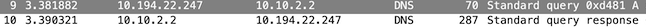
\includegraphics{dns.png}
\\
\end{figure}\\
The first packet is a DNS query and the next is the query response corresponding to that sent from the DNS server. The whole process took approximately 8.5 ms. 

\subsection{HTTP filter}
The HTTP messages sent/received are as in the figure when the webpage was requesting using \texttt{Google Chrome}. There are approximately 25  request  messages and 25 response messages.
\begin{figure}[h]
\centering
\caption{HTTP messages}
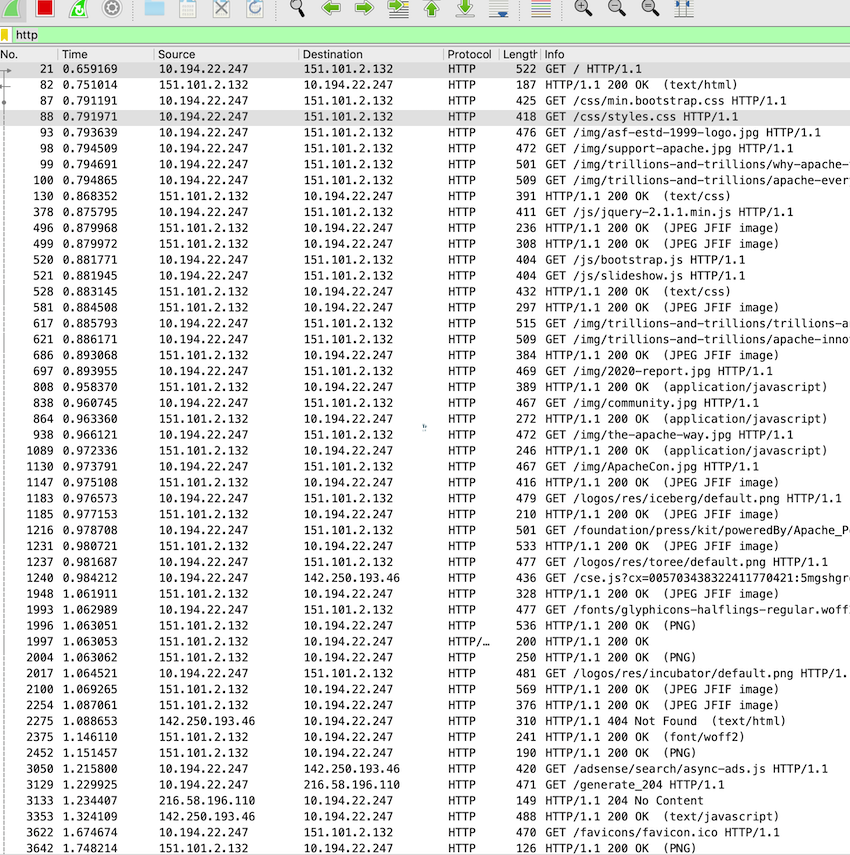
\includegraphics{http.png}
\\
\end{figure}
\begin{enumerate}
    \item Observe that the text, images, the Javascript and CSS of the webpage, all are retrieved separately. 
    \item Also, when the webpage was fetched using the \texttt{wget} command, the only HTTP messages visible were the first \texttt{GET} message and the next response message corresponding to the base HTML file.
    \item This shows that the different components of the webpage, the text, graphics, the fonts etc are all stored in separate files in the server. 
\end{enumerate}
\textbf{The browser first downloads the base(mostly textual) HTML page. Apart from the text segment, it contains links to the various other objects such as the CSS file, the JS file and the images wherever necessary. As the web browser renders the HTML page, it encounters the links to these files and requests for the same.}
\subsection{Time taken to load webpage}
The time taken to load the webpage was approx 1.18 seconds. It was calculated by subtracting the time when the first \texttt{GET} request was sent from the time when final HTTP response was received.
\subsection{Comparison with cse.iitd.ac.in}
The HTTP response to a query to iitd.ac.in was a message with code 301(Permanently moved). I tried it with \texttt{twitter.com} and \texttt{facebook.com}, both of them showed no activity under HTTP filter. \\
This is probably due to the fact that the websites use HTTPS rather than HTTP which is more secure and the files transferred over it are encrypted. The corresponding messages can be viewed under the SSL filter.
\section{Implementing \texttt{traceroute} using \texttt{ping}}

\subsection{Algorithm}
\begin{enumerate}
    \item The working of \texttt{traceroute} can be found on the man page for it. We implement it in a way similar to that. 
    \item We successively ping at the required domain name while incrementing the ttl value of the ping starting from 1. For each ping, if the ttl limit is reached, an error message is received that contains the IP address of the last reached router which can be parsed easily.
    \item In the other case, it might happen that the router does not respond to the ping at all. To handle that, we send multiple pings to the router to increase the probability of it responding. In case it does not respond at all. We declare a timeout and proceed to the next ttl value.
    \item The script can be run by \texttt{python2} \texttt{traceroute.py} \textless\texttt{domain-name}\textgreater
\end{enumerate}
\subsection{Output and plots}
The following is the output for \texttt{www.iitd.ac.in}.The machine was connected to IITD-WiFi.
\begin{center}
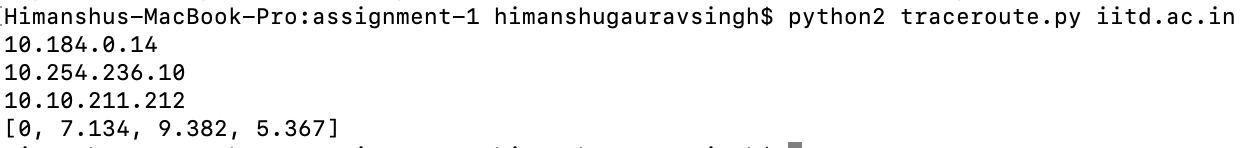
\includegraphics[width=\textwidth,height=\textheight,keepaspectratio]{iitd.ac.in.png}
\\
  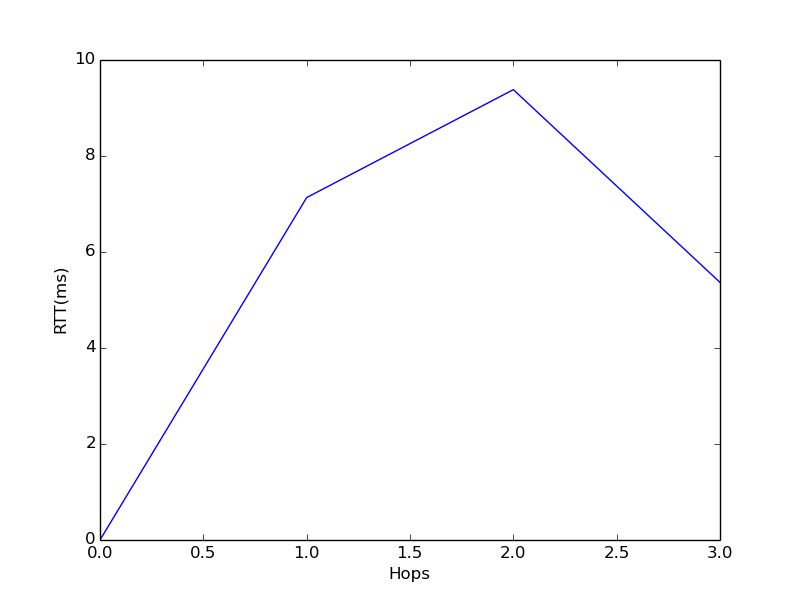
\includegraphics[width=\textwidth/2,height=\textheight/2,keepaspectratio]{traceroute_iitd.ac.in.png}
\\
\end{center}

The following is the output for \texttt{www.facebook.com}.The machine was connected to an Airtel-hotspot. \\
\begin{center}
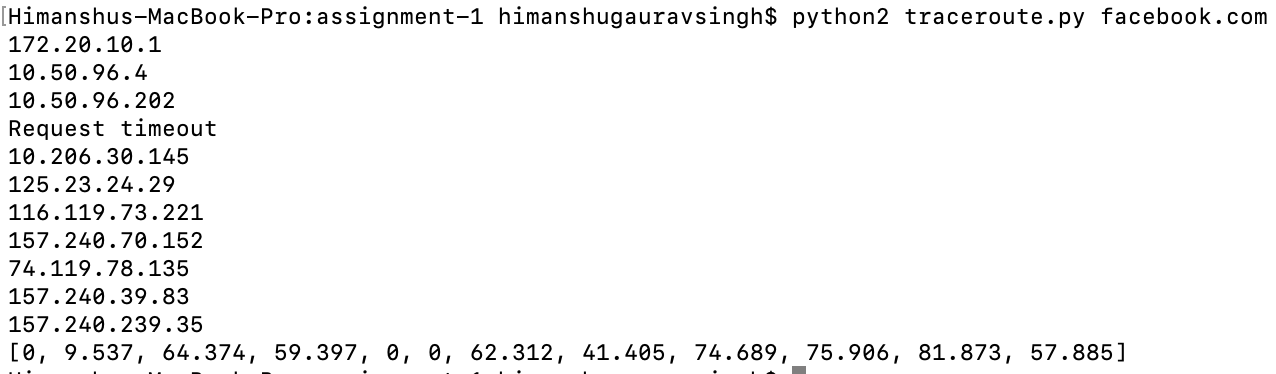
\includegraphics[width=\textwidth,height=\textheight,keepaspectratio]{facebook.png}
\\
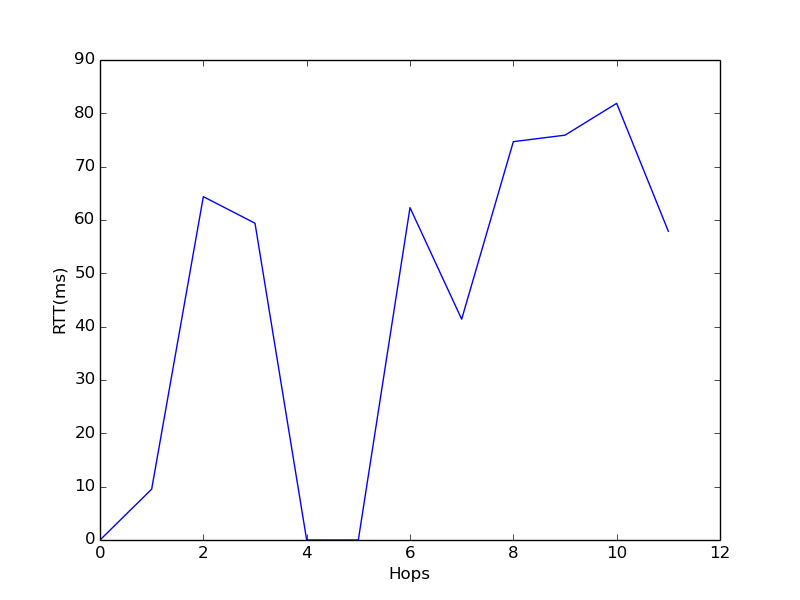
\includegraphics[width=\textwidth/2,height=\textheight/2,keepaspectratio]{traceroute_facebook.com.png}
\\
\end{center}

\subsubsection{Observation}
\begin{enumerate}
    \item Observe that the plots are not strictly increasing as might be expected. This is probably due to variable latency of the routers and end-systems over time and for different pings. 
    \item Several of the routers do not respond back to the sender, causing a time-out response. Also, this behaviour is not consistent over multiple runs. 
\end{enumerate}

\end{document}
